\section{Kopplingsschema över sensorenhet}

\begin{figure}[h]
\center
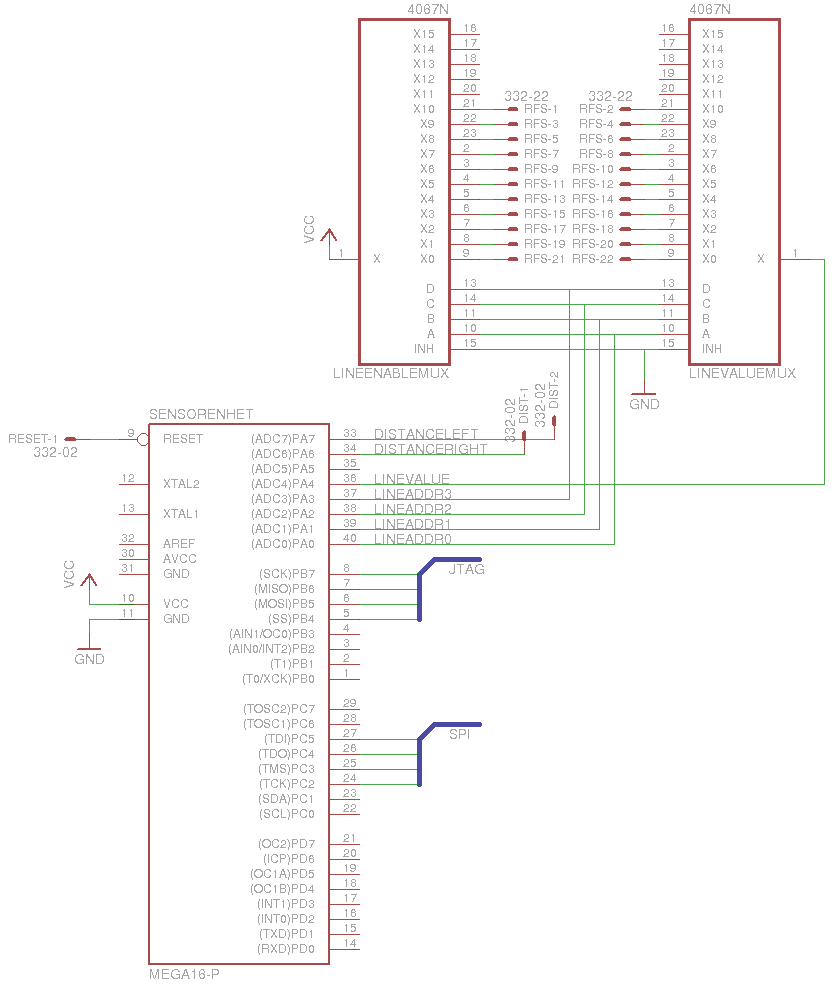
\includegraphics{sensorenhet}
\caption{Kopplingsschema över sensorenhet}
\end{figure}

RESET-1 är en avstudsad tryckomkopplare som ger negativ flank vid nertryckning. Signalerna RFS går till reflexsensormodulen. Jämna nummer är utsignaler från fototransistorerna. Udda är enablesignaler till lysdioderna. DISTANCELEFT och DISTANCERIGHT är utsignalerna från avståndssensorerna. LINEADDR-signalerna kontrollerar vilken lysdiod i reflexsensormodulen som är aktiv. SPI-bussen ansluts till huvudenheten. JTAG-bussen kopplas till JTAG ICE-3.
